\documentclass{article}
\usepackage{graphicx}
\usepackage{titletoc}
\usepackage{titlesec}
\usepackage{geometry} 
\usepackage{fontspec, xunicode, xltxtra}
\usepackage{float}
\usepackage{cite}
\usepackage{amsmath}
\usepackage{amssymb}
\usepackage{listings}
\usepackage{titletoc}
\usepackage{bm}
\usepackage{multirow}

\geometry{left=3cm,right=3cm,top=3cm,bottom=3cm}
\DeclareMathOperator*{\argmin}{argmin}
\DeclareMathOperator*{\argmax}{argmax}
\DeclareMathOperator*{\var}{var}
\DeclareMathOperator*{\expec}{E}

\begin{document}
\title{\textsf{Course Project for Pattern Recognition}}
\author{Fan JIN\quad (2015011506)}
\maketitle

\tableofcontents
\clearpage

\section{Introduction and Preprocessing}
{
    Here is a glance at the datasets. 
    Columns with only one unique value are removed, as they have no effect as observations.
    The training set is roughly 9 times as much size as the testing set.

    \begin{table}[!hbp]
        \centering
        \begin{tabular}{|c|c|c|c|}
        \hline
        File & sample size (nrow) & number of features (ncol) & number features in effect \\
        \hline
        2ctrainX.txt & 2298 & 25133 & 17951 \\
        \hline
        2ctestX.txt & 256 & 25133 & 17951 \\
        \hline
        10ctrainX.txt & 16074 & 25133 & 24307 \\
        \hline
        10ctestX.txt & 1787 & 25133 & 24307 \\
        \hline
        \end{tabular}
        \caption{Shape of datasets}
    \end{table}

    \begin{itemize}
        \item For two-category classification, the response ``2ctrainY.txt'' takes values 1 and 2.
        \item For ten-category one, the response ``10ctrainY.txt'' takes values ranging from 1 to 10.
    \end{itemize}
}

\section{Two-category classification}
{
    \subsection{Feature selection}
    {
        Feature selection is neccesary in this case, for we have much more features than data points, referred to as the ``large p, small n'' problem.

        Methods of feature selection include:
        \begin{itemize}
            \item Non-wrapping: Fisher-based
            \item Non-wrapping: Correlation-based
            \item Non-wrapping: Entropy-based
            \item Non-wrapping: Statistical t-distribution
            \item Non-wrapping: Principal Component Analysis (PCA)
            \item Wrapping: Foreward-backward recursive
            \item Stochastic: Genetic algorithm
        \end{itemize}

        Here we use non-wrapping methods for feature selection. We chose Fisher-based and PCA.

        \subsubsection{Fisher criterion}
        {
            The fisher criterion is defined as 
            $$F = \frac{(\mu_1 - \mu_2)^2}{s_1^2 + s_2^2},$$
            where $\mu_1$, $\mu_2$ are the means of two categories, and $s_1^2$, $s_2^2$ are the varainces, in terms of some feature.

            The larger the Fisher criterion, the more significant the feature is. We select 2000 features with the largest Fisher criteria. 
        }

        \subsubsection{the PCA}
        {
            The Principal Component Analysis performs eigendecomposition to the correlation matrix of the data points, and retains the components with principal eigenvalues.

            We retain 99\% of total variance in raw data, which gives $2202$ features in total. 
        }
    }

    \subsection{Classifier}
    {
        \subsubsection{Linear SVM}
        {
            The support vector machine, or SVM, is a powerful method for both classification and regression, particularly in case of ``large p, small n''.

            It is crucial to choose a kernel that balances between prediction accuracy and overfitting aversion. 
            We tried linear, quadratic, and RBF kernels. The linear kernel turns out the best.
        }

        \subsubsection{Fully connected NN}
        {
            The neural network has advantages over the linear SVM in case of nonlinearity. 

            Since we have only limited data points, we cannot train a deep network. 
            We took a simple perceptron network, which has one hidden layer with 1500 nodes. 
            We tuned the hidden layer size, and $1000$ proves the best hyperparameter.
        }
    }

    \subsection{Experiments}
    {
        \begin{table}[!hbp]
            \centering
            \begin{tabular}{|c|c|c|c|c|c|c|c|}
            \hline
            Dim. Reduction & Classifier & \multicolumn{5}{|c|}{5-fold cross validation} & Avg. Accuracy \\
            \hline
            Fisher & Linear SVM & 0.9848 & 0.9934 & 0.9869 & 0.9869 & 0.9956 & 0.9896 \\
            \hline
            PCA & Linear SVM & 0.9544 & 0.9434 & 0.9629 & 0.9586 & 0.9498 & 0.9539 \\
            \hline
            Fisher & FC NN & 0.9891 & 0.9978 & 0.9891 & 1.0000 & 0.9956 & 0.9943 \\
            \hline
            PCA & FC NN & 0.8828 & 0.8652 & 0.8823 & 0.9019 & 0.8758 & 0.8816 \\
            \hline
            \end{tabular}
            \caption{Comparison}
        \end{table}

        The Fisher criterion has better performance in dimensionality reduction, compared with the PCA. 

        It is worth noting that the neural network does not always perform better than the SVM. 
        It does when we use Fisher criterion for dimensionality reduction, while it does not when the PCA is used. 
        This could be explained by the weak performance of the PCA, as it performs a linear transformation on the raw data.
        The data might not be normally distributed, and thus the correlation matrix fails to identify all the principal components.

        We tuned the hyperparamters, and found the best network size is around 1000. This attains high accuracy while avoiding overfitting.

        \begin{table}[!hbp]
            \centering
            \begin{tabular}{|c|c|c|c|c|c|c|}
            \hline
            Size of hidden layer & \multicolumn{5}{|c|}{5-fold cross validation} & Avg. Accuracy \\
            \hline
            200 & 0.9934 & 0.9978 & 0.9934 & 0.9847 & 0.9934 & 0.9925 \\
            \hline
            500 & 0.9891 & 0.9978 & 0.9891 & 1.0000 & 0.9934 & 0.9939 \\
            \hline
            1000 & 0.9891 & 0.9978 & 0.9891 & 1.0000 & 0.9956 & 0.9943 \\
            \hline
            1500 & 0.9891 & 0.9978 & 0.9891 & 1.0000 & 0.9956 & 0.9943 \\
            \hline
            \end{tabular}
            \caption{Finding the proper network size}
        \end{table}
    }

    \subsection{Prediction}
    {
        Since it has the highest accuracy in 5-fold cross validation, the fully connected NN with Fisher-based dimensionality reduction is chosen for prediction. 
        The prediction is stored in ``2ctestY.txt'' in the root directory.
    }
}

\section{Ten-category classification}
{
    \subsection{Feature selection}
    {
        The dataset is too large for SVD (singular value decomposition), so it would be diffucult to perform full PCA on it.
        We tried using ``arpack'' instead, but the script ran out of memory on a GPU server. 

        Considering this, only Fisher criterion was used in this task.
        We chose 2000 features out of 24307, and trained the reduced dataset using SVM and FCNN.
    }

    \subsection{Experiments}
    {
        \begin{table}[!hbp]
            \centering
            \begin{tabular}{|c|c|c|c|c|c|c|c|}
            \hline
            Dim. Reduction & Classifier & \multicolumn{5}{|c|}{5-fold cross validation} & Avg. Accuracy \\
            \hline
            Fisher & Linear SVM & 0.9916 & 0.9878 & 0.9850 & 0.9903 & 0.9875 & 0.9884 \\
            \hline
            Fisher & FC NN & 0.9891 & 0.9950 & 0.9937 & 0.9925 & 0.9934 & 0.9927 \\
            \hline
            \end{tabular}
            \caption{Comparison}
        \end{table}

        The fully connected NN attains higher accuracy as the linear SVM does. 

        \begin{table}[!hbp]
            \centering
            \begin{tabular}{|c|c|c|c|c|c|c|}
            \hline
            Size of hidden layer & \multicolumn{5}{|c|}{5-fold cross validation} & Avg. Accuracy \\
            \hline
            200 & 0.9934 & 0.9925 & 0.9875 & 0.9940 & 0.9931 & 0.9921 \\
            \hline
            500 & 0.9546 & 0.9928 & 0.9931 & 0.9934 & 0.9866 & 0.9841 \\
            \hline
            1000 & 0.9953 & 0.9944 & 0.9944 & 0.9937 & 0.9937 & 0.9943 \\
            \hline
            1500 & 0.9959 & 0.9940 & 0.9944 & 0.9947 & 0.9940 & 0.9946 \\
            \hline
            \end{tabular}
            \caption{Finding the proper network size}
        \end{table}

        The optimal hyperparameter for the hidden layer size is around 1000. 

        Compared with two-category classification, the ten-category one attains slightly lower accuracy in training and cross validation.

    }

    \subsection{Prediction}
    {
        Since it has the highest accuracy in 5-fold cross validation, the fully connected NN with Fisher-based dimensionality reduction is chosen for prediction. 
        The prediction is stored in ``10ctestY.txt'' in the root directory.
    }
}

\section{Visualization and Clustering}
{
    \subsection{PCA}
    {
        \begin{figure}[H]
            \centering
            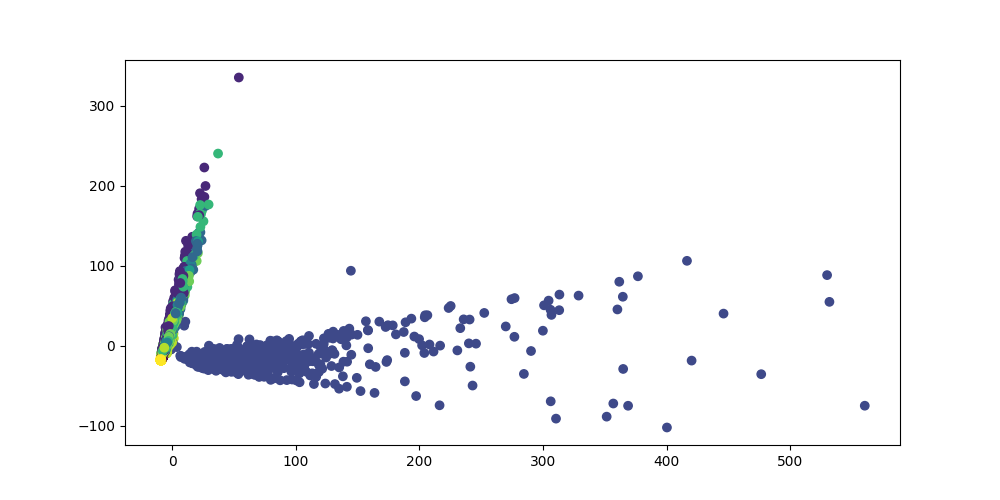
\includegraphics[width = 1\linewidth]{./src3/pca.png}
            \caption{Dimensionality reduction using PCA}
        \end{figure}
    }

    \subsection{t-SNE}
    {
        \begin{figure}[H]
            \centering
            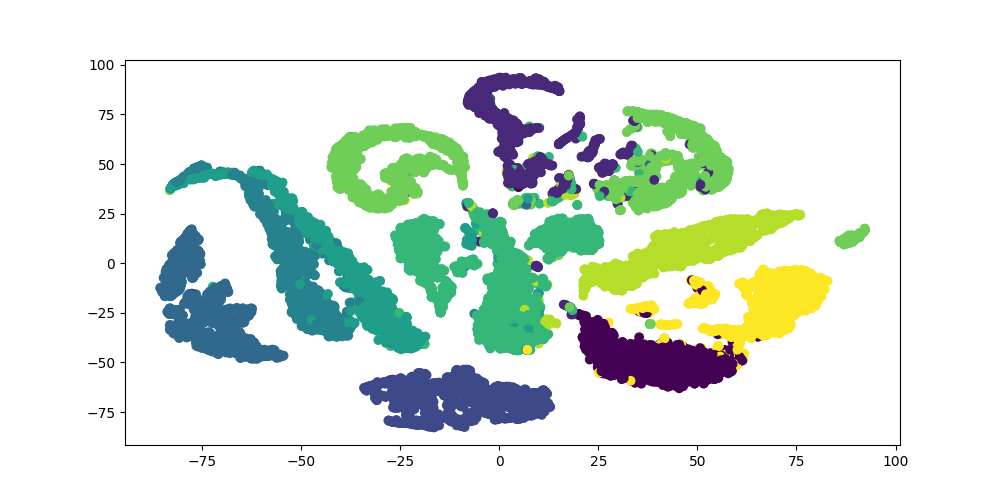
\includegraphics[width = 1\linewidth]{./src3/tsne.png}
            \caption{Dimensionality reduction using t-SNE}
        \end{figure}
    }

    \subsection{Clustering based on t-SNE}
    {
        It is astouding to find the result of PCA, although with good linearity, does not split up all the 10 categories in the 2d space.
        Only one category is distributed away from others. In comparison, the t-SNE works fine. We will use t-SNE for clustering.

        Since the number of categories is known, k-means seems a good choice. We fix $k=10$. 
        The birch clustering algorithm is also tested. The Birch algorithm turns out better than K-means.

        \begin{table}[!hbp]
            \centering
            \begin{tabular}{|c|c|}
            \hline
            Method & Accuracy \\
            \hline
            K-means & 0.6926 \\
            \hline
            Birch & 0.7343 \\
            \hline
            \end{tabular}
            \caption{Comparison}
        \end{table}

        \begin{figure}[H]
            \centering
            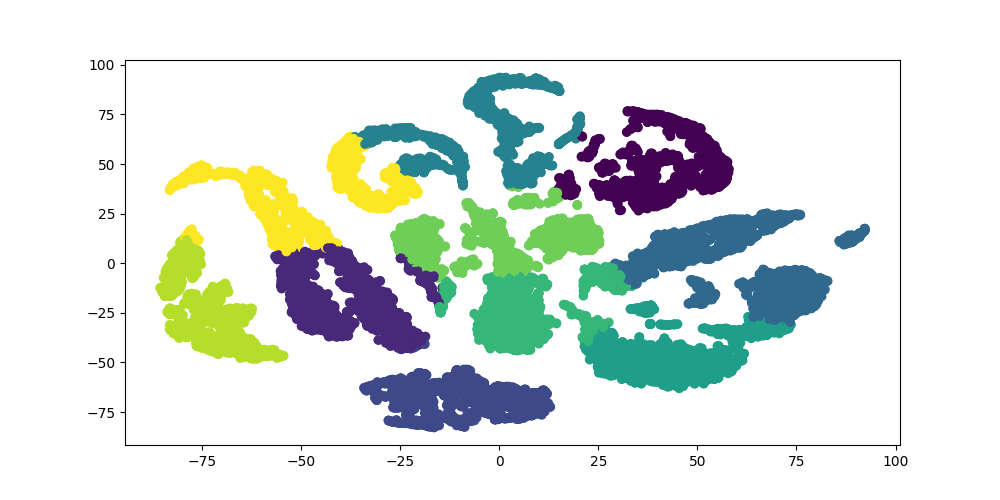
\includegraphics[width = 0.9\linewidth]{./src3/kmeans.png}
            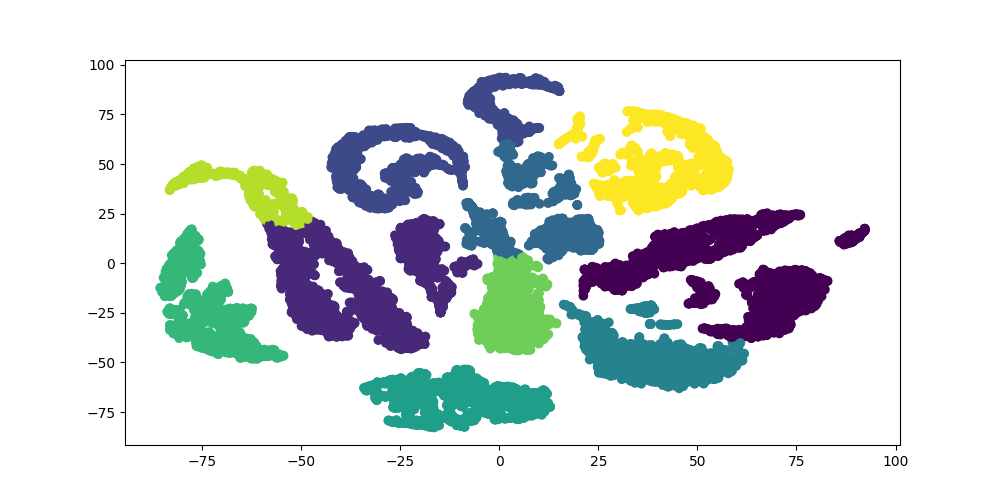
\includegraphics[width = 0.9\linewidth]{./src3/birch.png}
            \caption{K-means (top); Birch (bottom)}
        \end{figure}
    }
}

\section{Source Code}
{
    \subsection{Root directory}
    {
        \begin{itemize}
            \item ``2ctestY.txt'': Two-category prediction. Use this file for evaluation.
            \item ``10ctestY.txt'': Ten-category prediction. Use this file for evaluation.
            \item ``report.pdf'': Project report.
        \end{itemize}
    }

    \subsection{``data1'' directory}
    {
        \begin{itemize}
            \item ``2ctrainX.txt'': Raw dataset.
            \item ``2ctrainY.txt'': Raw dataset.
            \item ``2ctestY.txt'': Raw dataset.
            \item ``data1.npz'': Preprocessed file. (invalid columns removed)
        \end{itemize}
    }

    \subsection{``data2'' directory}
    {
        \begin{itemize}
            \item ``10ctrainX.txt'': Raw dataset.
            \item ``10ctrainY.txt'': Raw dataset.
            \item ``10ctestY.txt'': Raw dataset.
            \item ``data2.npz'': Preprocessed file. (invalid columns removed)
        \end{itemize}
    }

    \subsection{``src1'' directory}
    {
        \begin{itemize}
            \item ``preproc.py'': Preprocessing, removing identical columns.
            \item ``feature\_selection'': Feature selection, generating ``fisher\_2000.npz'' and ``pca\_99.npz''.
            \item ``SVM.py'': Training a SVM and use it for prediction.
            \item ``FCNN'': Training a fully connected NN and use it for prediction.
        \end{itemize}
    }

    \subsection{``src2'' directory}
    {
        \begin{itemize}
            \item ``preproc.py'': Preprocessing, removing identical columns.
            \item ``feature\_selection'': Feature selection, generating ``fisher\_2000.npz''.
            \item ``SVM.py'': Training a SVM and use it for prediction.
            \item ``FCNN'': Training a fully connected NN and use it for prediction.
        \end{itemize}
    }

    \subsection{``src3'' directory}
    {
        \begin{itemize}
            \item ``pca.py'': Dimensionality reduction by PCA, generating ``pca.npz''.
            \item ``tsne.py'': Dimensionality reduction by t-SNE, generating ``tsne.npz''.
            \item ``visualization'': Visualization after loading ``pca.pna'' and ``tsne.npz''. 
            \item ``kmeans.py'': Clustering by K-means.
            \item ``birch.py'': Clustering by Birch.
        \end{itemize}
    }
}

\clearpage
\end{document}
    